\chapter{Analysis}
\minitoc
\label{Cap:Analysis}
%++++++++++++++++++++++++++++++++++++++
%     Introduction 
%++++++++++++++++++++++++++++++++++++++

\section{Introduction}
\label{Cap:Analysis:Introduction}
In the \textbf{Subsection} \ref{Cap:Int:Motivation} the reasons to continue with the studies of the 1$\pi^+$ production in MINER$\nu$A experiment are explained. In this section, the the process for the calculation of the one differential cross section (1D analysis) and a double differential cross section (2D analysis) for 1 pion production are shown. The results of the cross sections are shown in the \textbf{Chapter} \ref{Cap:xSec}. The signal definition for both is the same. The innovation for these analyses is that two different techniques of data selection are used, these are explained in \textbf{subsections} \ref{Cap:Analysis:DataSelection:Cuts:Tracked} and \ref{Cap:Analysis:DataSelection:Cuts:UntrackedPions}. 

The measurement of the 1D analysis respect to $x$ variable is obtained as follow:

\begin{equation}
    \left(\frac{d\sigma}{dx}\right)_i= \beta \frac{\Sigma_{j}U_{ij}(N^{data}_j - N^{simBkgd}_j)}{\epsilon_{i}\phi T\Delta x_i}
    \label{eq:difXSec}
\end{equation}

Where $j$ is the bin of the $x$ reconstructed variable, $i$ is the bin of the $x$ true variable, $N_j^{data}$ is the selected data for the reconstructed $j$ bin, $N_j^{sim Bkgd}$ is the simulated background for the reconstructed $j$ bin, $U_{ij}$ is the unfolding matrix, $\beta$ is the material correction factor, $\epsilon_i$ is the simulated efficiency of data selection and acceptance correction for the $i$ true bin, $\phi$ is the neutrino flux, $T$ is the number of target nuclei in the detector and $\Delta x_i$ is the bin width for the variable $x$ for the $i$ true bin.

For the case of the 2D analysis respect to the variable $x$ and $y$ is obtained as follow:

\begin{equation}
    \centering
    \left(\frac{d^2\sigma}{dxdy}\right)_{ij}= \beta \frac{\Sigma_{ab}U_{abij}(N^{data}_{ab} - N^{simBkgd}_{ab})}{\epsilon_{ij}\phi T\Delta x_{i}y_j}
\end{equation}

The measurement for the 2D analysis is similar to the 1D analysis, where $a$ and $b$ are the reconstructed bins for the $x$ and $y$ variables respectively, $i$ and $j$ are the true bins for the $x$ and $y$ variables respectively, $N_j^{data}$ is the selected data, $N_j^{sim Bkgd}$ is the simulated background, $U_{ij}$ is the unfolding matrix, $\beta$ is the material correction factor, $\epsilon_i$ is the simulated efficiency of data selection and acceptance correction, $\phi$ is the neutrino flux, $T$ is the number of target nuclei in the detector $\Delta x_i y_j$ is the bin width for the variable $x$ for the $i$ true bin.

In the way to compare the data, the MC models and the MC reconstruction simulation, there are three categories of data:
\begin{itemize}
    \item \textit{Data}: it corresponds to the reconstructed information obtained directly from the detector.
    \item \textit{MC}: It is the information obtained from the reconstructed interactions in the detector simulation, more details in \textcolor{red}{hacer referencia a la reconstruction}. 
    \item \textit{True}: it corresponds to the information obtained directly from the neutrino interaction simulation, it includes information obtained directly from the models, systematic errors of the models, particles ID, etc. More details in \ref{Cap:Simulation:GENIE}.
\end{itemize}

The information obtained from the \textit{MC} and \textit{true} data allows to simulate the background, to estimate the detector efficiency, to apply different cuts, to estimate the purity of the sample, to tune the background and compare the data directly with the models. 

In the following bullets are explained the steps to measure the cross section, for the 1D and 2D analysis cases:

\begin{enumerate}
    \item \textbf{Signal Definition and analysis variables:} This is the first stage of the analysis, in this stage is defined the physical process that will be studied. Here are studied the constrains for the analysis delimited by the detector capabilities and the variables respect to the differential cross section will be obtained. In the \textbf{sections} \ref{Cap:Analysis:SignalDefinition} and \ref{Cap:Analysis:Variables} are shown the specific signal definition and variables that will be used for the analyses. 

    \item \textbf{Data Selection:} At this stage, according to the signal definition, cuts are applied to the data set. To apply these cuts the data is passed event by event looking for characteristics that satisfy the requirements of the signal definition, at the same time the events that do not pass the cuts are removed. In the selected events set there are signal and background events. The signal events are the events that pass the cuts and satisfy the signal definition, by other hand the background corresponds to the events that pass the cuts but these do not correspond to the signal definition. From the MC simulation the signal and background events can be identify using the information obtained from the simulation process, but not in the data case. In this stage the simulated purity and efficiency are used to optimize the data selection. 

    The purity is calculated as follow:
    \begin{equation}
        purity=\frac{Signal\ Events}{Signal+Background\ Events}
        \label{eq:Analysis:Purity}
    \end{equation}
    The purity brings information about the fraction of the simulated data that really corresponds to the signal definition. During the data selection process it is essential to improve, remove or apply cuts in the way to perform the data selection.

    For the efficiency, it is calculated as 
    
    \begin{equation}
        \epsilon=\frac{Signal\ Events}{True\ Signal\ Events}
        \label{eq:Analysis:efficiency}
    \end{equation}
    where the \textit{True Signal Events} corresponds to the total number of simulated events that match the signal definition. 
    In the \textbf{Section} \ref{Cap:Analysis:DataSelection} the results for the data selection are shown. 

    \item \textbf{Background subtraction:} In this step, the simulated background is removed from the data and MC data selection. One question about this procedure is how well is simulated the background, trying to have a better approximation to the real background in the experiment the \textit{Sideband} studies are developed to make the \textit{background tuning}. The sideband studies consist to apply the data selection but in space face region where most part of the events are characterized to be background, it basically consist to remove one of the cuts that are applied during the data selection. In this region the simulation is fitted respect to the data. After to fit the background it is subtracted bin by bin to the data selection, giving as result the data selection histogram with out the background shape. 

    \item \textbf{Unfolding:} The detector is not perfect, there are many sources of uncertainties associated to the energy reconstruction, vertex reconstruction, particle identification, etc. These imperfections smear the data selection distributions. The unfolding procedure remove this smearing from the data selection. This can be interpreted as the unfolding transform the histogram from a reconstructed space to a true space where the detector is perfect. 

    \item \textbf{Efficiency correction:} During the data selection process there are events that do not pass the cuts because the inefficiency of the cuts. To repopulate the histograms with the lost events $\epsilon_i$ is used, $i$ is the true bin number. $\epsilon_i$ is obtained as in the \textbf{equation} \ref{eq:Analysis:efficiency} but for each bin. 

    \item \textbf{Normalization:} This is the last step on the cross section measurement, for this last part the efficiency corrected distributions are normalized by the number of protons and neutrons in the detector region (fiducial volume), the flux of neutrinos and the bin width to obtain the differential cross section. 
    
\end{enumerate}

    In the following sections present the results for each step of the differential and double differential cross section measurements. For these results the data POT is 1.05689$\times 10^{21}$ and the MC POT is 4.37033$\times 10^{21}$.  The variables used for the analysis are described in the \textbf{Section} \ref{Cap:Analysis:Variables}.


\section{Analysis Variables}
\label{Cap:Analysis:Variables}

\subsection{One differential cross section}
\label{Cap:Analysis:Variables:1DAnalysis}

The one differential cross section is obtained respect to the variables presented in the \textbf{Table} \ref{tab:Analisys:AnaVariables:1Danalysis}. For some variables, the central value of the variable depends if the event pass the cuts for an tracked pion or for a untracked pion. The cuts and the definitions for tracked and untracked pions are defined in the \textbf{Section} \ref{Cap:Analysis:DataSelection}.

\begin{table}[!htb]
    \centering
    \begin{tabular}{c|l}
        \hline
        Variable & Description \\ \hline
        $T_\pi$      & Pion kinetic energy. For this analysis the value of this variable is\\ 
                     & obtained by two methods. These two methods are described in the \\
                     & \textbf{Section} \ref{Cap:Analysis:SignalDefinition}. \\
        \hline
        $\theta_\pi$ & Pion polar angle respect to the neutrino beam direction. The central \\
                     & value of this variable depends if the event has a tracked or untracked \\
                     & pion. This is explained in the \textbf{Section} \ref{Cap:Analysis:DataSelection}. \\
        \hline
        $P_\mu$      & Muon momentum magnitude. The momentum of the muon is measured  \\
                     & by MINOS Near detector, the muon momentum can be reconstructed  \\
                     & by the track length or by curvature. The muon reconstruction is \\
                     & explained in \ref{Cap:MnvExp:MnvDetector:DataReconstruction}. \\
        \hline
        $\theta_\mu$ & Muon polar angle respect to the neutrino beam direction. This is \\
                     & measured by the MINER$\nu$A detector taking as origin the neutrino \\
                     & vertex position an the reconstruction algorithm measure the angle.\\
        \hline
        $P^z_\mu$    & Muon longitudinal momentum respect to the neutrino beam. It is \\ 
                     & obtained by $P^z_\mu = P_\mu cos \theta_\mu$. \\
        \hline
        $P^T_\mu$    & Muon transversal momentum respect to the neutrino beam. It is \\
                     & obtained by $P^T_\mu = P_\mu sin \theta_\mu$. \\
        \hline
        $E_\nu$      & Neutrino energy. This is estimated by the relation $E_\nu = E_\mu + E_{had}$. \\
                     & Where $E_\mu$ is the muon energy and $E_{had}$ is the estimated hadronical. \\
                     & energy. \\
        \hline
        $Q^2$        & Four-momentum transfer by the neutrino. Defined as $Q^2 = - (p_\nu -p_\mu)^2$\\ 
                     & or using lepton kinematics $Q^2 = 2E_\nu(E_\mu-P^z_\mu) + m^2_\mu$. Where $p_\nu$ and\\ 
                     & $p_\mu$ are the four-momentum of the incoming neutrino and the muon\\
                     & respectively.\\ 
        \hline
        $W_{exp}$    & Experimental invariant hadronic mass. $W_{exp} = m^2_N + 2m_NE_{had} - Q^2$ \\
                     & $= m^2_N + 2m_N(E_\nu-E_\mu)$ is used as approximation of W.\\
        \hline
    \end{tabular}
    \caption{Variables used in the 1D analysis and a description of each variable.}
    \label{tab:Analisys:AnaVariables:1Danalysis}
\end{table}

These are some clarifications that have to be given for $E_{had}$ and $W_{exp}$. $E_{had}$ is a variable that usually is smeared fro the real value, it is because in the interactions can be produced can be produced, which are invisible for the detector. Other sources of smearing are the production of pions, charged or neutral, and the initial state of the nucleons. For this analysis the hadronical energy is obtained by two methods, depending if the event pass the cut to be a categorized as pion tracked or untracked event. For the case of the tracked event $E_{had}$ is obtained as follow:

\begin{equation}
    E_{had} = T_\pi + m_\pi + E_{had,\ no\ \pi^+}
    \label{eq:EhadTracked}
\end{equation}

Where $m_\pi$ is the rest mass of the positive pion, $E_{had,\ no\ \pi^+}$ is the  no-pion-muon corrected remaining energy. To obtain $E_{had,\ no\ \pi^+}$, the first step is measure all the visible energy deposited by the final particles in the detector without the muon track energy. usually called $E_{avail}$, then, the calorimetric energy from the pion candidate tracks is removed, and finally is applied a calorimetric correction, all this process is fully described in \cite{AaronThesis}.  

By other hand, for the case when the event corresponds to an untracked pion event, the hadronical energy is calculated as follow: 

\begin{equation}
    E_{had} = N_{michels}m_\pi + E_{avail}
    \label{eq:EhadUntracked}
\end{equation}

Where $N_{michels}$ is the number of michel electrons observed, $m_\pi$ is the rest mass of the pion and $E_{Avail}$ is the available energy. This definition is made with the assumption that untracked pion events do not necessary exhibit a pion track, although a pion is produced, hence the rest mass of the pion must be considered in the $E_{had}$ measurement. $E_{avail}$ is obtained as follow: 

\begin{equation}
    E_{avail} = \beta_{avail\ Scale}(E_{recoil\ Tracker} + E_{recoil\ ECAL)}
\end{equation}

where $\beta_{avail\ Scale}$ is a calorimetric scale that is always equal to 1.17 \textcolor{red}{Preguntar sobre alguna referencia para el 1.17 y el muon fuzz}, $E_{recoil\ Tracker}$ is the reconstructed energy in the tracker removing the muon deposited energy and the muon fuzz energy, the muon fuzz energy correspond to the small tracks produced around to the muon track, and the $E_{recoil\ ECAL}$ that corresponds to the energy reconstructed in the ECAL without the muon track and muon fuzz energy.

The theoretical invariant mass (W) is calculated by $W^2=(p_\nu+p_N+p_\mu)^2$, where $p_\nu$, $p_N$ and $p_\mu$ are the neutrino, nucleon and muon four-moment respectively. In the experiments $p_\nu$ and $p_N$ can not be measured directly. However, in the experiments is commonly used $W_{exp}$ as approximation using variables that can be estimated. In this analysis to obtain the $w_{exp}$ the two definitions of $E_{had}$ are used, it depends of the cuts that the event pass.  

\subsection{Double differential cross section}
\label{Cap:Analysis:Variables:2DAnalysis}

In a 2D analysis are combined 2 variables to have a more detailed description of the neutrino interactions. The combinations used for this analysis are $T_\pi$ vs $P_\mu$, $T_\pi$ vs $P^T_\mu$, $P^z_\mu$ vs $P^T_\mu$ and $E_\nu$ vs $T_\pi$.

\textcolor{red}{Aqui hay que clarificar cual es el tipo de variables que se van a utilizar, si vamos a agergar los untrack pion a la data selection y comentar que se usan los mismos costes que para el analisis en 1D, tal vez una direrente data selection para thetpi, pero creo que si se puede agregar esa variable, de igual forma que $E_\nu$ vs $T_\pi$}

%++++++++++++++++++++++++++++++++++++++
%     Signal definition 
%++++++++++++++++++++++++++++++++++++++

\section{Signal Definition}
\label{Cap:Analysis:SignalDefinition}

The signal definition delimits the interest physical process for the analysis. Here, the interaction types and the space phase are defined depending of the detector capabilities.

Essentially, in this thesis is treated one signal definition that is the production of one charge pion events by muon-neutrino charge current interaction in the MINER$\nu$A tracker, writing in the condensed formula $CC\ \nu_\mu+CH\xrightarrow{}\pi^+ + X + \mu$. Where $CH$ corresponds to the plastic scintillator of the tracker, $\pi^+$ one positive charge pion, $X$ corresponds to a nucleon (proton or neutron) but not other mesons and $\mu$ that corresponds to the muon. There are other conditions that are no described in the condensed formula, these will be explained below. 

According to the physical progress defined above the selected events must to be produced by CC muon-neutrino interactions, producing only one charged pion without other mesons for a $W_{exp} <$ 1.4 GeV. $W_{exp}$ is limited with the intention to measure meanly events where $\Delta$ (1232) is produced, it also reduce the multi-pion events, the production of neutral particles that can not be detected directly and as $W_{exp}$ increase is more difficult to measure the out coming particles kinematics. 

There are other limits applied to the signal definition due the detector capabilities, such as 1.5 GeV $<P_\mu<20$ GeV, $\theta_\mu<20$ GeV, vertex position in the MINER$\nu$A tracker region, and there are \textcolor{red}{Cuantas condiciones tenemos, por el momento solamente pondr\'e las del analysis 1D} different condition for $T_\pi$:
\begin{itemize}
    \item $0<T_\pi<350$ MeV, this condition is applied for the 1D analysis when $\theta_\pi$ is not included in the measurement.  
    \item $20<T_\pi<350$ MeV, this condition is applied for the 1D analysis when the variable $\theta_\pi$ is analyzed. 
\end{itemize}

The $T_\pi$ upper limit is impose because the pions with a higher energy leave the detector, and the pions can not be reconstructed. The reason why there is an special signal definition for $\theta_\pi$ is because for the untracked pion events, $\theta_\pi$ is estimated by the polar angle between the neutrino direction and the position of the closest michel electron end point, using as reference the neutrino vertex interaction. This measurement is a good approximation to the real $\theta_\pi$ for a region of the pion kinetic energy, however, it is necessary to make an analysis of the region where the pion angle is not well reconstructed. In the \textbf{Figure} \ref{fig:Analysis:SignalDefinition:1DAnalysis:thetapivsTpi}. From the migration matrices, the discrepancy between the reconstructed and true $\theta_\pi$ is observed for $T_\pi < 20$ MeV region. For this reason it was decided to restrict $T_\pi$ only when $\theta_\pi$ is measured. 

The restriction for $P_\mu>1.5$ GeV is imposed because below this momentum, the muon does not have enough momentum to reach the MINOS detector, and above of 20 GeV the muon is going out of MINOS and the momentum can not be measured by curvature. The restriction for $\theta_\mu < 20$\textdegree is due to the fact that it seeks to guarantee that the muon will leave MINER$\nu$A backwards and enter MINOS detector.

The analysis is focused to look for interactions in the tracker region, the fiducial volume defined for the Z axis in the detector coordinate system is 5990 cm $< z <$ 8340 cm with a transversal hexagonal area of 850 cm measured from the center of the detector. This region excludes the target upstream region, the downstream calorimeters, the OD around the tracker region. 

For the 2D analysis the signal definition is similar to the 1D analysis. For the 2D analysis, the data selection does not include the untracked pion events, hence $T_\pi$ is limited to the region 35 MeV $<T_\pi<$ 350 MeV. The lower limit is impose because the tracked pions can not pass through more that 5 planes, it is an reconstruction condition for the short tracks to be reconstructed. 


\begin{figure}[!htb]
    \centering
    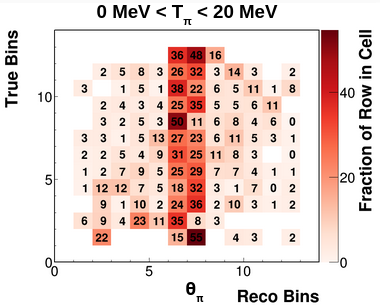
\includegraphics[scale=0.33]{Figures/Chapter4/SignalDefinition/thetapi0to20tpi.png}
    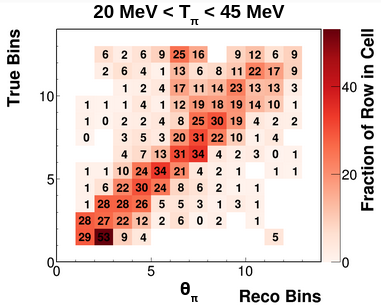
\includegraphics[scale=0.33]{Figures/Chapter4/SignalDefinition/thetapi20to45tpi.png}
    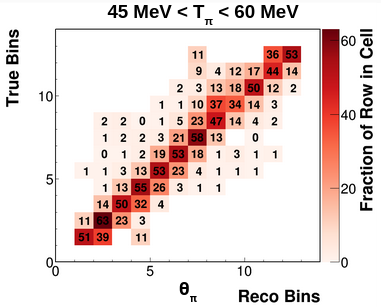
\includegraphics[scale=0.33]{Figures/Chapter4/SignalDefinition/thetapi45to60tpi.png}
    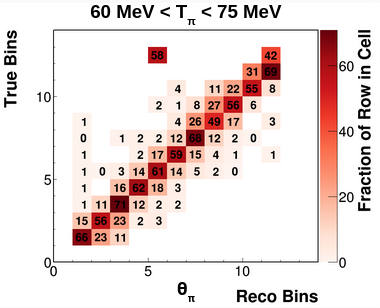
\includegraphics[scale=0.33]{Figures/Chapter4/SignalDefinition/thetapi60to75tpi.png}
    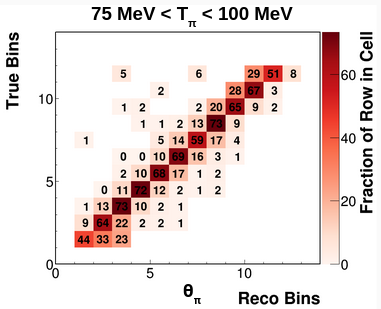
\includegraphics[scale=0.33]{Figures/Chapter4/SignalDefinition/thetapi75to100tpi.png}
    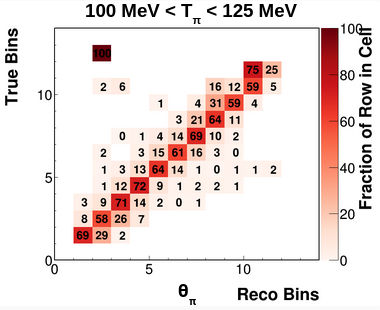
\includegraphics[scale=0.33]{Figures/Chapter4/SignalDefinition/thetapi100to125tpi.png}
    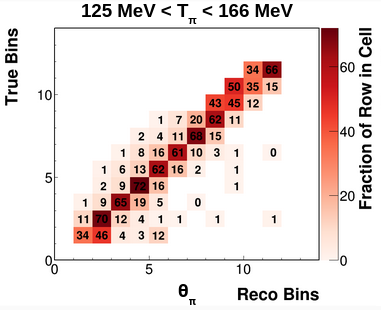
\includegraphics[scale=0.33]{Figures/Chapter4/SignalDefinition/thetapi125to166tpi.png}
    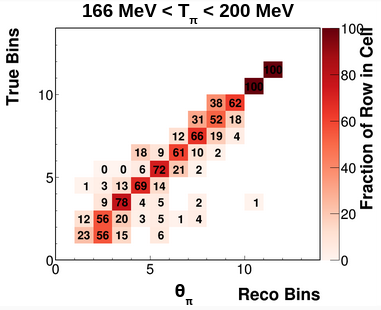
\includegraphics[scale=0.33]{Figures/Chapter4/SignalDefinition/thetapi166to200tpi.png}
    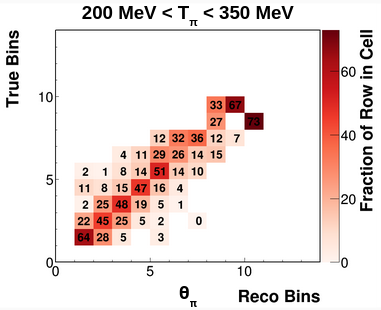
\includegraphics[scale=0.33]{Figures/Chapter4/SignalDefinition/thetapi200to350tpi.png}
    \caption{Migration matrices for $\theta_\pi$ for different regions of True $T_pi$. The bad reconstruction of $\theta_\pi$ for $0<t_\pi<20$ MeV is shown. The $\theta_\pi$ binning showed in the plots does not correspond to the real binning, it just a homogeneous binning used to have a better perception of the migration matrix. The $\theta_\pi$} binning used for this analysis is [0., 15., 30., 45, 60, 75., 90., 105., 120., 135., 150., 165., 180.].
    \label{fig:Analysis:SignalDefinition:1DAnalysis:thetapivsTpi}
\end{figure}


%++++++++++++++++++++++++++++++++++++++
%     Data Selection 
%++++++++++++++++++++++++++++++++++++++
\section{Data Selection}
\label{Cap:Analysis:DataSelection}

In this section are described the cuts that are applied to obtain the data selection for the 1D and 2D analyses. Here are shown the cut tables for the events that pass the cuts showing the efficiency and purity of the data selection. The signal definition described in the \textbf{Section} \ref{Cap:Analysis:SignalDefinition} delimit what kind of events should be included in the data selection. In the data selection the quantities that must be optimized are the purity and the efficiency. The way to increase the purity is increasing the cuts or restrictions applied to the data set, but it reduce the efficiency of the data selection at the same time that increase the statistical error. 

In particular this analysis uses two different data selection techniques, which are named tracked pion data selection and untracked pion data selection. The reasons for that is used this mixed data selection is explained in \ref{Cap:Int:Motivation}.


\subsection{Cuts}
\label{Cap:Analysis:DataSelection:Cuts}

The cuts are classified in three types. The \textit{General cuts}, \textit{tracked Pion cuts} and the \textit{Untracked Pion cuts}. The general cuts are applied to the tracked and untracked pion events. The general cuts are:

\begin{itemize}
    \item \textbf{Vertex position Cut}: This cut removes all the events where the interaction vertex is no produced in the fiducial volume defined in the signal definition. In this analysis, the interaction must be produce in the tracker region. \textcolor{red}{Checar con ben si el fiducial volume deber ser igual para la data selection que para signal definition}
    \item \textbf{Muon Cuts}: In signal definition it is required that the incident neutrino must have a muon-neutrino and it have to interact by charge current interaction, for this reason the events must to have an observable muon track and it also has to reach the MINOS detector and produce a muon with a curvature that corresponds to a negative muon. This cut remove the Neutral Current (NC) interaction events and the muon charge sign removes the events that are coming from $\overline{\nu_\mu}$. 
    
    The other muon cuts remove the events where the reconstructed muon has a $\theta_\pi<$ 20\textdegree and when $P_\mu < 1.5$ GeV and $P_\mu>$ 20 GeV, the reasons why these cuts are applied are the same that the conditions imposed in the signal definition.  
    \item \textbf{$\pi^0$ Cut}: This cut removes the events where $\pi^0$ are produced. The $\pi^0$ can not be observed directly, however, these decay very fast producing two gammas. In the detector it is observed as isolated energy clusters generated out of the vertex interaction position with a limit of time of \(\sim\) 30 ns after the neutrino interaction. This cut increse the purity around of 9\% and has a cut efficiency of the 95\%.\textcolor{red}{agregar mas informacion acerca de los cortes como la eficiencia o la pureza y tal vez algunas graficas de los cortes
    }. 
\end{itemize}


\subsubsection{Tracked pions}
\label{Cap:Analysis:DataSelection:Cuts:Tracked}

These are the cuts typically applied in the charge pion analyses in the \textbf{Section} \ref{Cap:Int:Motivation}. For this analysis, most part of the cuts are applied and these are described in the following bullets: 

\begin{itemize}
    \item \textbf{At least one hadron track:} At least one track that does not correspond to the muon track must be observed in the vertex. These tracks are considered as candidate hadron tracks and must undergo the hadron quality cuts. The hadron track quality cuts check whether the hadron track is forked, exiting, produced in the side ECAL, matches the OD, and is produced in the tracker. The Forked cut is impose to remove the events where the hadron interacts with the detector creating other tracks making it difficult to measure the hadron energy. The exiting cut removes the events where the hadron track is not contained in the ID region, hence is not possible to measure the total hadron energy. The side ECAL matches the OD cuts removes the events where hadron is going to the side ECAL or to OD. The last cut, checks if the reconstructed hadron is contained in the tracker.
    \item \textbf{At lest 1 matched michel electron:} The 99.9\% of the $\pi^+$ decays in the way $\pi^+\xrightarrow{}\mu^+ + \nu_\mu$ with a life time of $\tau \sim$ 26 ns, after the $\mu^+$ decays as $\mu^+\xrightarrow{} e^+ + \overline{\nu}_\mu + \nu_e$ with a life time $\tau\sim$ 2.2 \(\mu\)s, the $e^+$ produced is known as michel electron. The michel electron is observed as a track spatial separated and time-delayed from the interaction neutrino vertex. 

    Based on the previous description of the michel electrons, the selection of the michel electrons is performed by initially searching for hit clusters produced in time slices after the neutrino interaction. The distance between the vertex and the cluster must not exceed 50 cm, and the energy of the michel electron must be consistent with the energy expected from the muon decay process.  

    The next step is to associate the michel electron with a hadron track. The first step is to measure the distance between the michel electron and the endpoint of the hadron track. The subsequent step involves categorizing the michel electron into the following types: \textit{fitted}, \textit{Unfitted}, and \textit{One-view}. The michel electron's category depends on the number of detector planes it traverses. A michel electron falls into the fitted category when it passes through multiple planes, and its track can be reconstructed as a line. For this category, the distance is measured between the endpoint of the hadron track and the closest endpoint of the michel electron track. In the case of the unfitted category, the michel electron passes through at least 2 planes. For this case, the distance is measured from the endpoint to the cluster's energy-average mean position. In the last case, the michel electron falls into this category when it only deposits energy in just one plane, and the distance is measured similarly to the unfitted category. 

    Depending of the category are imposed maximum distances, for the fitted = 7.5 cm, unfitted = 50 cm and one-view = 50 cm. In the cases of multiple hadron tracks it takes closer candidate to the michel electron, giving a pion candidate.
    \item \textbf{Particle Identification (PID) score:} After to get the pion candidate, the PID cut removes the events where the track is confused and it does not correspond to a pion-like track profile.
    
    During the reconstruction process, the algorithm initially identifies the muon track and assumes that the remaining tracks correspond to either a proton or a charged pion. To each track is estimated the energy-loss per unit of length of the charged particle when it pass through matter, more commonly know as $\frac{dE}{dx}$. These $\frac{dE}{dx}$ is compared with the $\frac{dE}{dx}$ profile of a proton and a charge pion, obtained by the Bethe-Bloch formula \cite{DetectionTechniques}. Each particle has a particular $\frac{dE}{dx}$ profile. The MINER$\nu$A Bethe-Bloch curves for the proton and pion are shown in the \textbf{Figure} \ref{fig:Analysis:DataSelection:Cuts:dEdXBetheProfiles}. 


    \begin{figure}[!htb]
        \centering
        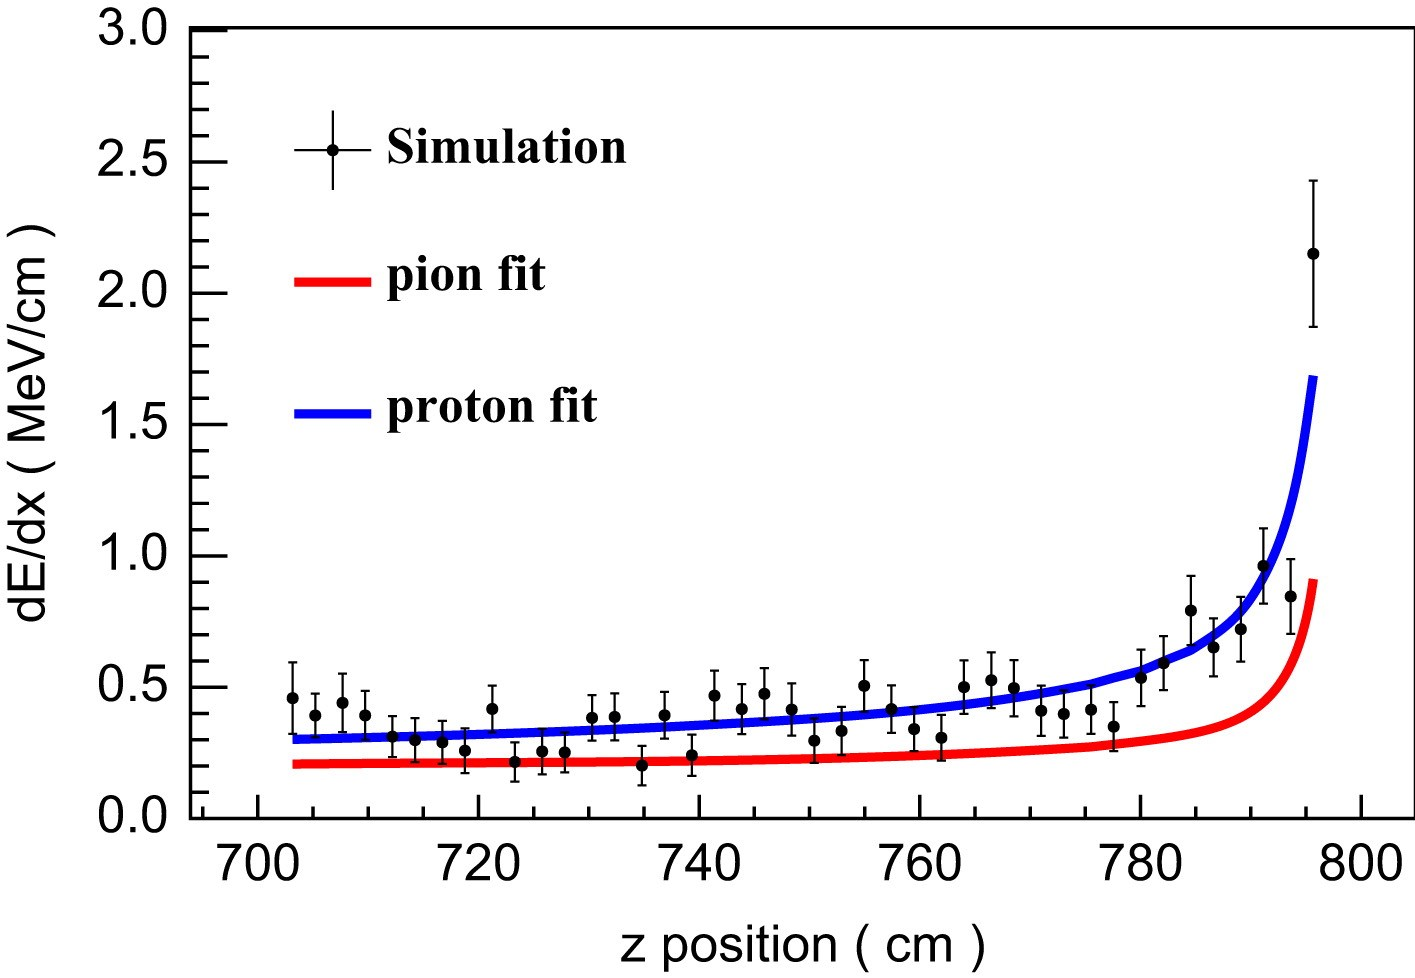
\includegraphics[scale=0.1]{Figures/Chapter4/DataSelection/dedxprotonSim.jpg}
        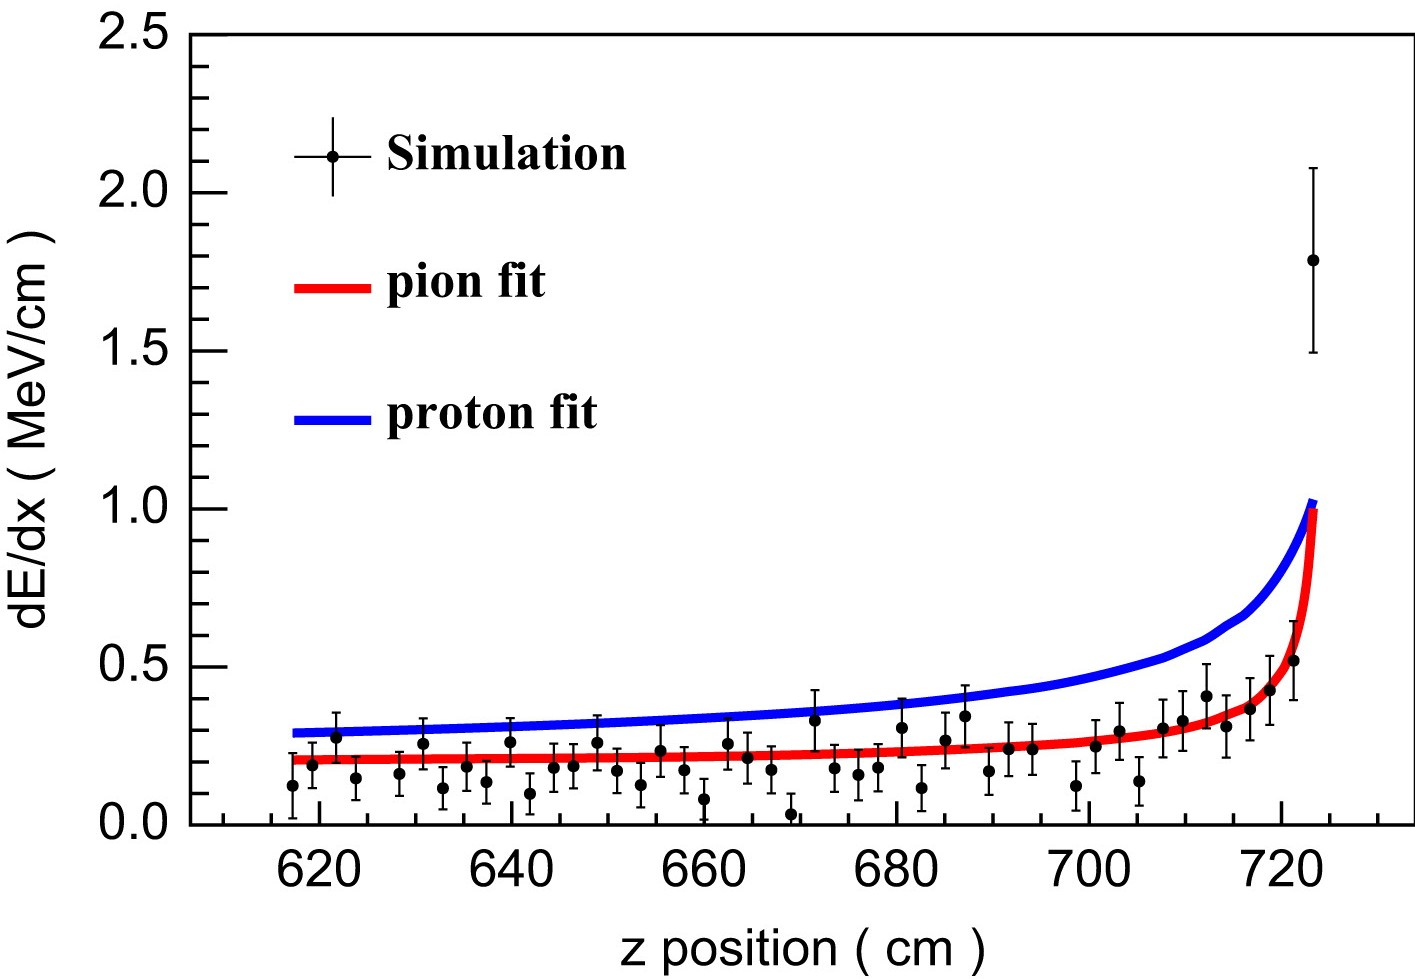
\includegraphics[scale=0.1]{Figures/Chapter4/DataSelection/dedxpionSim.jpg}
        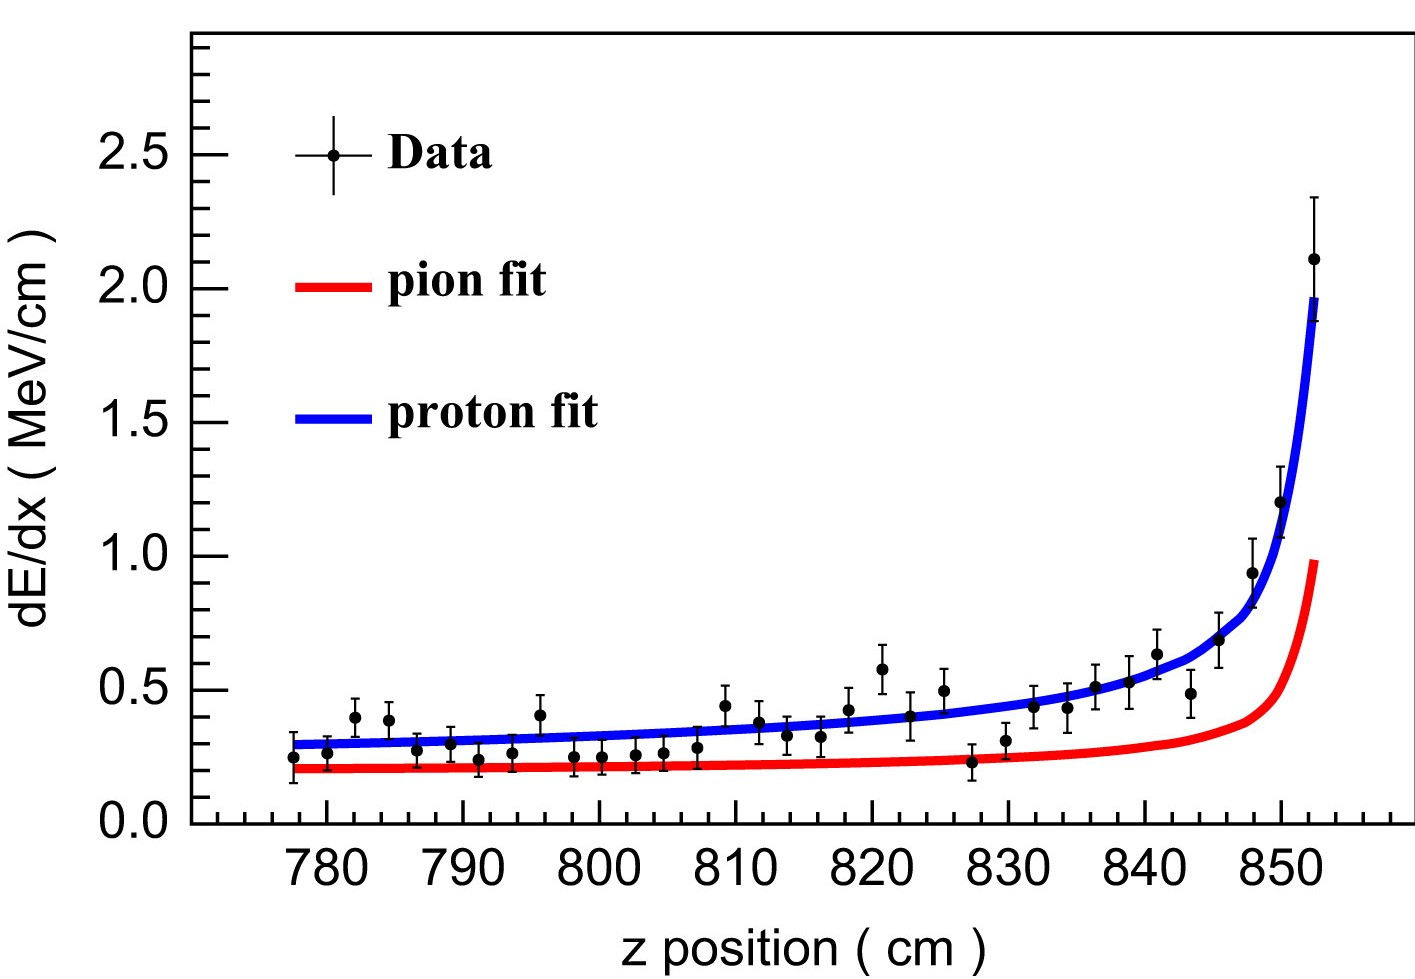
\includegraphics[scale=0.1]{Figures/Chapter4/DataSelection/dedxprotonData.jpg}
        \caption{The plots show the comparison of the Bathe-Bloch $\frac{dE}{dx}$ profiles for protons and pions with the simulated $\frac{dE}{dx}$ profiles for protons (top-left), pions (top-right) and for data taken using protons (bottom). Figures taken from \cite{ALIAGA2014130}.}
        \label{fig:Analysis:DataSelection:Cuts:dEdXBetheProfiles}
    \end{figure}

    To obtain the PID score of a track, each node of the track is compared with a likelihood function template that was created using a large set of simulated protons and pions. This was done using a Monte Carlo (MC) gun, varying the angle and energy of the particles. The likelihood template calculates the probability by assessing the fraction of pion or proton tracks with a node of identical energy at the same position along the track. The likelihood function $\mathcal{L}$ is formed as the product of all these individual probabilities as follow:
    \begin{equation}
        \mathcal{L}\left(particle|track\right)=\prod_{Nodes}P\left(E_{Node}|particle\right)
    \end{equation}

    Using the log of the Neyman-Pearson lemma \cite{Neyman-Pearson} to obtain the most optimal criteria to distinguish between the particle hypothesis, called PID score, is obtained by

    \begin{equation}
        PID\ Score = \sum_{Node} (logP(E_{node}|\pi)-logP(E_{node}|p))
        \label{eq:Analysis:Cuts:PID}
    \end{equation}

    For the cases where there are overlapped tracks close to the interaction vertex, the PID score is not a reliable metric, for this reason when is observed that in a track the energy in a node falls more that 1.9737 MeV between two node in the first 10 nodes the high-energy nodes are removed from the PID calculation. The Bethe-Bloch equations assumes that the particles is stopped in the material, it means that the particle does not interact inelastically with the material. For this reason in the likelihood calculation are included these effects and the maximum likelihood is used. 

    This analysis is focused on pion, hence in the \textbf{Equation} \ref{eq:Analysis:Cuts:PID} the PID score $>$ 0 corresponds to a major probability that track corresponds to a pion. \textcolor{red}{Agregar una grafica con el LLR score antes de aplicar el corte}

    
    \item \textbf{End nodes energy:} This cut is used to remove the events where the pion candidate interacts with the detector inelastically, because the energy usually is not well reconstructed for this kind of events. A bad reconstruction of this quantity implies a bad reconstruction of other variables such as $E_\nu$, $W_{exp}$ and $Q^2$. 

    When a particle travel though matter losing energy by ionization radiation, the $\frac{dE}{dx}(x)$ presents a pronounced peak before the particle comes to rest. This peak is know as the Bragg peak \cite{BraggCurves}. It must to be observed as increase of deposited energy at the end of the hadron track. 

    For the cases where the particle interacts inelastically with the detector, the Bragg peak is not observed. Therefore, events in which the pion candidate does not exhibit the Bragg peak are removed of the data selection. The Bragg peak for the proton presents a higher increase increase compared with to the peak generated by a pion, therefore this cut also applies an upper limit removing events where the chosen track does not correspond to a pion. 

    This cut checks the deposited energy in the last 6 nodes of the pion candidate track. The \textbf{Table} \ref{tab:Analysis:Cuts:EndnodeCuts} shows the ranges of energy per end-node that the pion candidate track must to have.  

    \begin{table}[]
        \centering
        \begin{tabular}{c|c}
            End Node & Energy Range (MeV)\\ \hline
            0+1      & (6, 32) \\
            2        & (2, 22) \\
            3        & (0, 19) \\
            4        & (0, 31) \\
            5        & (0, 60) \\
        \end{tabular}
        \caption{Acceptable ranges for last nodes of the end of each track.}
        \label{tab:Analysis:Cuts:EndnodeCuts}
    \end{table}
    
    \textcolor{red}{Mostar una imagen dode se muestran como afectan estos cortes, probablemente una imagen de como se ven los endnodes}

    
    \item \textbf{Pion Multiplicity:} This cut removes the events where there more that 1 pion track candidate. This cut also removes the events where $T_\pi < 35$ MeV and $T_\pi > 350$ MeV. 
    \item \textbf{$W_{exp}$ tracked cut:} This cut removes all the event that have an $W_{exp} > 1.4$ GeV. The reasons why this cut is applied are already explained in the signal definition \ref{Cap:Analysis:SignalDefinition}. The measurement of $W_{exp}$ requires $E_{had}$, for this cut is used the $E_{had}$ obtained by the procedure explained in \ref{Cap:Analysis:Variables} for the tracked pions. 
    
\end{itemize}

In \ref{tab:Analysis:Cuts:TrackedCutTable} the cut table for tracked cuts is shown. In this cut table is only included the tracked pion efficiency and purity. This table was obtained using only the ME1A playlist of the data set of MINERvA. In the table the general cuts are applied too. 

\begin{sidewaystable}[!hbt]
    \tiny
    \centering
    \begin{tabular}{|*{12}{l|}}


    \hline
    & \multicolumn{4}{c|}{Signal} & \multicolumn{2}{c|}{Background} & \multicolumn{2}{c|}{Total} & \multicolumn{3}{c|}{Data} \\
    \hline
& N     & Eff     & Cut Eff & Pur    & N         & Eff     & N         & Eff     & N MC (scale) & N Data    & Data/MC \\\hline

 No Cuts   & 203952.17     & 100.00\% & 100.00\% &   1.12\% & 17978780.42 & 100.00\% & 18182732.59 & 100.00\% & NA & NA & NA \\ \hline
 Anatool Precuts   & 159558.28     &  78.23\% &  78.23\% &   5.62\% & 2677126.18 &  14.89\% & 2836684.46 &  15.60\% & NA & NA & NA \\ \hline
 vertex position Cut   & 156840.33     &  76.90\% &  98.30\% &   5.79\% & 2551834.64 &  14.19\% & 2708674.97     &  14.90\% & 598128.93     & 676952.00 &   1.13 \\ \hline
 MINOS Muon   & 151236.27     &  74.15\% &  96.43\% &   9.77\% & 1396389.62 &   7.77\% & 1547625.89     &   8.51\% & 341746.36     & 358090.00 &   1.05 \\ \hline
 1.5 GeV $<$ Pmu $<$ 20 GeV   & 150525.85     &  73.80\% &  99.53\% &  10.12\% & 1336621.79 &   7.43\% & 1487147.65     &   8.18\% & 328391.57     & 342163.00 &   1.04 \\ \hline
 $\theta_{\mu}$ $<$ 20 degrees   & 150457.23     &  73.77\% &  99.95\% &  10.30\% & 1310983.53 &   7.29\% & 1461440.76     &   8.04\% & 322714.99     & 335784.00 &   1.04 \\ \hline
 $<$2 Isolated Prongs   & 134544.17     &  65.97\% &  89.42\% &  17.94\% & 615463.26 &   3.42\% & 750007.43     &   4.12\% & 165616.45     & 173567.00 &   1.05 \\ \hline
 $>$= 1 Hadron Track   & 77042.84     &  37.77\% &  57.26\% &  21.07\% & 288531.88 &   1.60\% & 365574.72     &   2.01\% & 80726.12     & 82223.00 &   1.02 \\ \hline
 $>$= 1 Michel   & 25370.23     &  12.44\% &  32.93\% &  42.89\% & 33787.16 &   0.19\% & 59157.39     &   0.33\% & 13063.12     & 12876.00 &   0.99 \\ \hline
 LLR PID   & 19359.43     &   9.49\% &  76.31\% &  45.58\% & 23117.93 &   0.13\% & 42477.35     &   0.23\% & 9379.84     & 9141.00 &   0.97 \\ \hline
 Node   & 15028.78     &   7.37\% &  77.63\% &  50.04\% & 15005.18 &   0.08\% & 30033.96     &   0.17\% & 6632.09     & 5991.00 &   0.90 \\ \hline
 Pion Multiplicity   & 15027.89     &   7.37\% &  99.99\% &  50.18\% & 14920.42 &   0.08\% & 29948.32     &   0.16\% & 6613.18     & 5984.00 &   0.90 \\ \hline
 $Tracked W_{exp}$   & 13709.32     &   6.72\% &  91.23\% &  67.31\% & 6657.79 &   0.04\% & 20367.11     &   0.11\% & 4497.46     & 4055.00 &   0.90 \\ \hline
    \end{tabular}
    \caption{Cut table for tracked events. DataPOT: 89785235631482617856.00. MCPOT: 406599660544667287552.00.}
    \label{tab:Analysis:Cuts:TrackedCutTable}
\end{sidewaystable}



\pagebreak

\subsubsection{Untracked pions}
\label{Cap:Analysis:DataSelection:Cuts:UntrackedPions}
The implementation of these cuts aims to increase the efficiency of the data sample, expanding the $T_\pi$ range without compromising purity. This data selection is grounded in the observation that 99\% of charged pions decay to produce a muon, which subsequently emits a Michel electron. With this in mind, it becomes feasible to identify pions by counting the number of Michel electrons generated after the neutrino interaction, even in the absence of a discernible pion track. Assuming that the muon produced by the pion decay travels in the same direction as the primary pion and that the distance between the Michel electron and the vertex is correlated with $T_\pi$, it becomes possible to mitigate the dependency on the pion candidate track having a new data selection. 

To understand the data selection process it is important to define the following quantities:
\begin{itemize}
    \item \textbf{Interaction vertex}: It corresponds to the reconstructed neutrino interaction position in the 3D space. 
    \item \textbf{Michel Cluster}: These are the clusters that are produced time slices after the neutrino interaction. The michel cluster endpoint have to be well reconstructed. 
    \item \textbf{Closest Michel endpoint:} For the michel cluster must be produced two endpoint. The distance between the vertex and these endpoints is measured, then the closest endpoint is selected.
    \item \textbf{Pion range:} It is the 3D distance between the interaction vertex and the closest endpoint.
    \item \textbf{Non-muon cluster:} this is a reconstructed cluster that it is not associated to a muon. It could be a pion, proton or other charged particle track. 
\end{itemize}
\begin{figure}
    \centering
    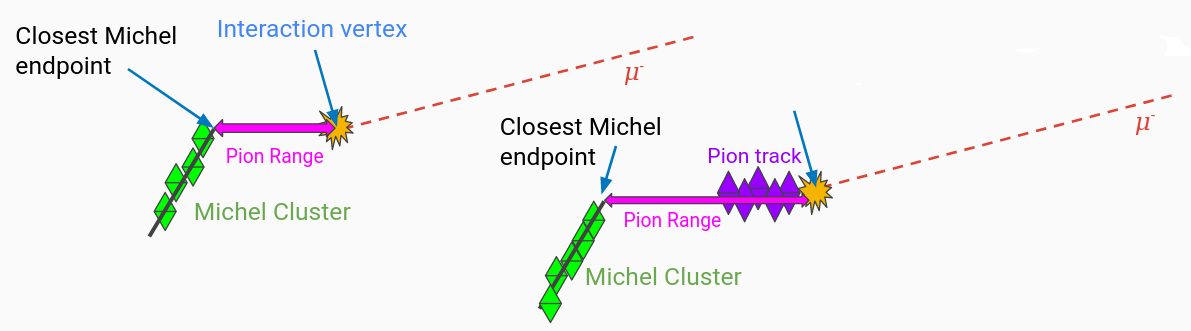
\includegraphics[scale=0.33]{Figures/Chapter4/DataSelection/TracklessPions.png}
    \caption{Scheme with two examples of pion events that can be produced part of the data selection, in the left, an event where the pion track is no produced but a michel electron is observed. The right scheme, it shows an event where is produced the track of a pion. }
    \label{fig:Analysis:Cuts:Untracked:MichelEventSheme}
\end{figure}

The cuts applied for the trackless pion are:

\begin{itemize}
    \item \textbf{Fitted Michel:} This cut eliminates all events where the Michel electron cluster is not reconstructed as fitted. As described earlier, Michel electron clusters fall into the fitted category when they traverse multiple planes, and the endpoints of the Michel electron are well reconstructed. Instances where unfitted or one-view Michel electrons are observed are excluded from the selection. Additionally, this cut removes Michel electrons that are observed 400 ns after the neutrino interaction. The output of this cut includes the identified Michel electron candidates.

    \item \textbf{2D distance cut:} The 2D distance cut measures the distance between vertex and michel electron ($XZ_{vtx-e}$, $UZ_{vtx-e}$ or $VZ_{vtx-e}$) or non-muon cluster  and michel electron ($XZ_{cluster-e}$, $UZ_{cluster-e}$ or $VZ_{cluster-e}$) for each michel endpoint. If the the distance exceeds 150 mm in 2 views the michel does not pass the cut. 
    
    The distance between the two views respect to the vertex is obtained as follow:
    \begin{equation}
        XZ_{vtx-e} = \sqrt{(x_{vtx}-x_e)^2 + (z_{vtx}-z_e)},
    \end{equation}
        \begin{equation}
        UZ_{vtx-e} = \sqrt{(u_{vtx}-x_e)^2 + (z_{vtx}-z_e)}l,
    \end{equation}
        \begin{equation}
        VZ_{vtx-e} = \sqrt{(v_{vtx}-x_e)^2 + (z_{vtx}-z_e)}.
    \end{equation}

    And respect to the non-muon cluster:

    \begin{equation}
        XZ_{cluster-e} = \sqrt{(x_{cluster}-x_e)^2 + (z_{cluster}-z_e)},
    \end{equation}
        \begin{equation}
        UZ_{cluster-e} = \sqrt{(u_{cluster}-x_e)^2 + (z_{cluster}-z_e)},
    \end{equation}
        \begin{equation}
        VZ_{cluster-e} = \sqrt{(v_{cluster}-x_e)^2 + (z_{cluster}-z_e)}.
    \end{equation}

    Where $x_{vtx}$, $x_{cluster}$ and $x_{e}$ is the position in the X plane of the vertex, cluster and michel electron respectively, for the $u_{vtx}$, $u_{cluster}$, $u_{e}$, $v_{vtx}$, $v_{cluster}$, $v_{e}$, $z_{vtx}$, $z_{cluster}$ and $z_{e}$ it is similar, just respect the planes U, V and the Z axis.

    \textcolor{red}{Explicar por que se usa esta distancia y este corte}
    
    \item \textbf{Closer michel cluster:} This cut measure the 3D distance between the vertex and the endpoints of all the michel candidates that passed the previous cuts. It returns the closest endpoint to the vertex or cluster. This information is used to obtain the best 3D distance between the vertex and the closest michel endpoint, this distance is called pion range. 
    \item \textbf{One pion cut:} This cut removes the event that presents more that one michel electron candidate. In this way the multi-pion events are removed from the sample.
    \item \textbf{$W_{exp}$ untracked cut:} This cut removes the events with $W_{exp} > 1.4$ GeV. The $E_{had}$ is obtained different that for the tracked events, the definition for the untracked hadronical energy is explained in \ref{Cap:Analysis:Variables}.

\end{itemize}

The untracked event data selection gives a similar efficiency compared to the tracked data selection. It is around of the 7\% and a purity of 62\%. In the \textbf{Table} \ref{tab:Analysis:Cuts:UntrackedCutTable} the cut table for the untracked events is shown. 

\begin{sidewaystable}[!hbt]
    \tiny
    \centering
    \begin{tabular}{|*{12}{l|}}


    \hline
    & \multicolumn{4}{c|}{Signal} & \multicolumn{2}{c|}{Background} & \multicolumn{2}{c|}{Total} & \multicolumn{3}{c|}{Data} \\
    \hline
& N     & Eff     & Cut Eff & Pur    & N         & Eff     & N         & Eff     & N MC (scale) & N Data    & Data/MC \\\hline
 No Cuts   & 203952.17     & 100.00\% & 100.00\% &   1.12\% & 17978780.42 & 100.00\% & 18182732.59 & 100.00\% & NA & NA & NA \\ \hline
 Anatool Precuts   & 159558.28     &  78.23\% &  78.23\% &   5.62\% & 2677126.18 &  14.89\% & 2836684.46 &  15.60\% & NA & NA & NA \\ \hline
 vertex position Cut   & 156840.33     &  76.90\% &  98.30\% &   5.79\% & 2551834.64 &  14.19\% & 2708674.97     &  14.90\% & 598128.93     & 676952.00 &   1.13 \\ \hline
 MINOS Muon   & 151236.27     &  74.15\% &  96.43\% &   9.77\% & 1396389.62 &   7.77\% & 1547625.89     &   8.51\% & 341746.36     & 358090.00 &   1.05 \\ \hline
 1.5 GeV $<$ Pmu $<$ 20 GeV   & 150525.85     &  73.80\% &  99.53\% &  10.12\% & 1336621.79 &   7.43\% & 1487147.65     &   8.18\% & 328391.57     & 342163.00 &   1.04 \\ \hline
 $\theta_{\mu}$ $<$ 20 degrees   & 150457.23     &  73.77\% &  99.95\% &  10.30\% & 1310983.53 &   7.29\% & 1461440.76     &   8.04\% & 322714.99     & 335784.00 &   1.04 \\ \hline
 $<$2 Isolated Prongs   & 134544.17     &  65.97\% &  89.42\% &  17.94\% & 615463.26 &   3.42\% & 750007.43     &   4.12\% & 165616.45     & 173567.00 &   1.05 \\ \hline
 Untracked Has Michel   & 61589.97     &  30.20\% &  45.78\% &  26.57\% & 170212.12 &   0.95\% & 231802.09     &   1.27\% & 51186.48     & 52895.00 &   1.03 \\ \hline
 Best Michel Distance   & 39690.52     &  19.46\% &  64.44\% &  43.88\% & 50759.18 &   0.28\% & 90449.70     &   0.50\% & 19973.08     & 20120.00 &   1.01 \\ \hline
 Closest Michel   & 39510.24     &  19.37\% &  99.55\% &  44.69\% & 48889.80 &   0.27\% & 88400.04     &   0.49\% & 19520.47     & 19759.00 &   1.01 \\ \hline
 One michel   & 14772.73     &   7.24\% &  37.39\% &  48.88\% & 15450.34 &   0.09\% & 30223.08     &   0.17\% & 6673.85     & 6874.00 &   1.03 \\ \hline
 $T_\pi<$ 350 MeV   & 14766.17     &   7.24\% &  99.96\% &  49.42\% & 15111.12 &   0.08\% & 29877.29     &   0.16\% & 6597.50     & 6826.00 &   1.03 \\ \hline
 $Untracked W_{exp}$   & 14415.76     &   7.07\% &  97.63\% &  62.21\% & 8757.88 &   0.05\% & 23173.64     &   0.13\% & 5117.20     & 5150.00 &   1.01 \\ \hline
    \end{tabular}
    \caption{P4 Cut Table, Untracked data selection,\today. DataPOT: 89785235631482617856.00. MCPOT: 406599660544667287552.00..}
    \label{tab:Analysis:Cuts:UntrackedCutTable}
\end{sidewaystable}

\pagebreak

\subsubsection{Data selection combination}

The interest results from these analyses comes to the fusion of the data selections described above, when these two data selection are combined the efficiency from a \(\sim\) 6\% to \(\sim\) 12\% and a purity of 64\%. This combination also provides the opportunity to study a $T_\pi$ region that was not previously explored. 

When the two data selections are combined, the events that pass the cuts falls in one of three categories, \textit{Tracked Event}, \textit{Untracked Event} or \textit{Mixed Event}.
\begin{itemize}
    \item \textbf{Tracked Event}: it corresponds to an event that pass the tracked pion cuts but it fails the untracked pion cuts. In a tracked event, the $T_\pi$ and $\theta_\pi$ central values are obtained using the information from the reconstructed pion track. For variables depended of $E_{had}$ such as $W_{exp}$, $E_\nu$ and $Q^2$, $E_{had}$ is obtained by the \textbf{Equation} \ref{eq:EhadTracked}.
    \item \textbf{Untracked Event:} it corresponds to an event that pass the untracked pion cuts but it fails the tracked pion cuts. In a tracked event, the $T_\pi$ and $\theta_\pi$ central values are obtained using the information of the michel electron. The reconstruction of these quantities are explained in \ref{Cap:MnvExp:MnvDetector:DataReconstruction:Untrackedpions}. For variables depended of $E_{had}$ such as $W_{exp}$, $E_\nu$ and $Q^2$, $E_{had}$ is obtained by the \textbf{Equation} \ref{eq:EhadUntracked}.
    \item  \textbf{Mixed Event:} it corresponds to an event that pass tracked and untracked pion cuts. When an event falls in this category, the value of the central value of all the variables is obtained in the same way that a tracked event. 
\end{itemize}
The selection of the category is also explained in the flowchart of the \textbf{Figure} \ref{fig:Analysis:Cuts:Flowchart} 

\begin{figure}[!htb]
    \centering
    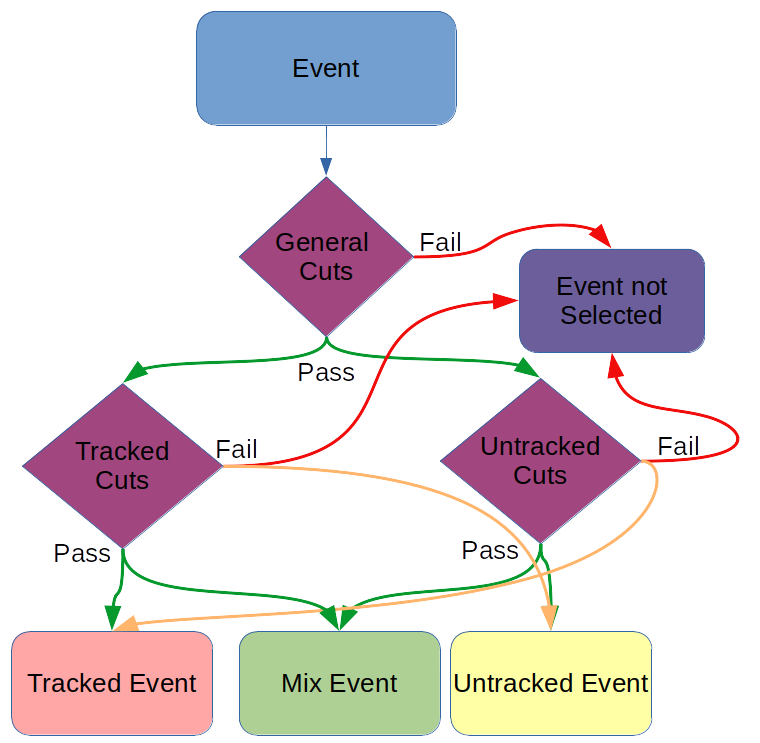
\includegraphics[scale=0.4]{Figures/Chapter4/DataSelection/EventSelFlowchart.png}
    \caption{Flowchart of of data selection for events when the tracked and untracked pions are included.}
    \label{fig:Analysis:Cuts:Flowchart}
\end{figure}

In the plot of the \textbf{Figure} \ref{fig:Analysis:Cuts:DataSelBreakdown}, this plot show the different data selection components. Is observed that for low-$T_\pi$ region the most representative category are the untracked events, as is expected. And conform the $T_\pi$ increase, the number of tracked events increase respect to the untracked. The percentage per category is shown in the \textbf{Table} \ref{tab:Analysis:Cuts:CategoryPercentage}.

\begin{figure}
    \centering
    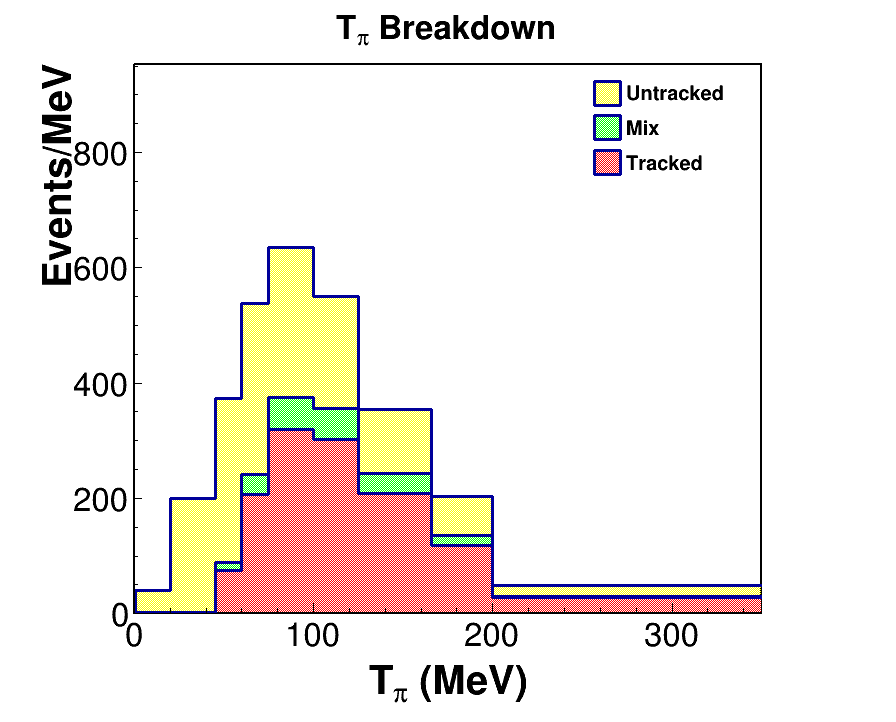
\includegraphics[scale=0.35]{Figures/Chapter4/DataSelection/Stacked_Tpi.png}
    \caption{Breakdown of data selection plot for the $T_\pi$ variable. The explains the category of the events.\textcolor{red}{Hacer una nueva grafica}}
    \label{fig:Analysis:Cuts:DataSelBreakdown}
\end{figure}

\begin{table}[!htb]
    \centering
    \begin{tabular}{c|c}
         Category  & Percentage (\%) \\ \hline
         Tracked   &  40.3 \\
         Untracked &  47.6\\
         Mix       & 12.1
    \end{tabular}
    \caption{Percentage of events per category.}
    \label{tab:Analysis:Cuts:CategoryPercentage}
\end{table}

\subsection{Data Selection 1D analysis Results}
\label{Cap:Analysis:DataSelectionResults1D}

The results that are shown here where obtained using the MINER$\nu$A data for the whole data set of the ME era, with the beam in the neutrino mode. The data POT is 1.0$\times 10^{21}$. For MC, is used GENIE v2.12.6, with the MINER$\nu$A tunes MnvGENIEv4.3.1+ Pion Reweight.The POT for MC is 4.90$\times 10^{21}$.



%\foreach \var in {loW,midW,hiW}{ 
\foreach \var in  {enu,mixtpi,mixthetapi_deg,pmu,ptmu,pzmu,thetamu_deg,q2,wexp}{
%\foreach \var in  {enu_true,mixtpi_true,pmu_true,ptmu_true,pzmu_true,thetamu_deg_true,q2_true,wexp_true}{
    \ifthenelse{\equal{\var}{enu}}{
      \renewcommand{\NewVar}{E_\nu}
    }{}
    \ifthenelse{\equal{\var}{mixtpi}}{
      \renewcommand{\NewVar}{T_\pi}
    }{}
    \ifthenelse{\equal{\var}{mixthetapi_deg}}{
      \renewcommand{\NewVar}{\theta_\pi}
    }{}
    \ifthenelse{\equal{\var}{pmu}}{
      \renewcommand{\NewVar}{P_\mu}
    }{}
    \ifthenelse{\equal{\var}{ptmu}}{
      \renewcommand{\NewVar}{P^T_\mu}
    }{}
    \ifthenelse{\equal{\var}{pzmu}}{
      \renewcommand{\NewVar}{P^z_\mu}
    }{}
    \ifthenelse{\equal{\var}{thetamu_deg}}{
      \renewcommand{\NewVar}{\theta_\mu}
    }{}
    \ifthenelse{\equal{\var}{q2}}{
      \renewcommand{\NewVar}{Q^2}
    }{}
    \ifthenelse{\equal{\var}{wexp}}{
      \renewcommand{\NewVar}{W_{exp}}
    }{}
    \begin{figure}
        \centering
        \includegraphics[scale=0.3]{Figures/Chapter4/DataSelection/Selection_\var__1Pi_untunedBG_BWN.png}
        \caption{$\NewVar$ 1D Data Selection.}
        \label{fig:Analysis:DataSelResults:\var}
    \end{figure}  
}

\subsection{Data Selection 2D analysis Results}
\label{Cap:Analysis:DataSelectionResults1D}

For the 2D analysis it only contains the tracked events, therefore the cut table that corresponds to this data selections \ref{tab:Analysis:Cuts:TrackedCutTable}. Fro this data selection is usesd the same data set that for the 1D analysis. For the simulation, the same simulation that for the 1D analysis was used. For this analysis the MC simulation is tuned by MnvGENIEv4.3.1, the Pion Reweighter is not applied because the trackless pions are not included in the data selection. 

%\foreach \var in {loW,midW,hiW}{ 
\foreach \var in  {ptmu_vs_tpi,pzmu_vs_ptmu,tpi_vs_pmu,tpi_vs_thetapi_deg}{
%\foreach \var in  {enu_true,mixtpi_true,pmu_true,ptmu_true,pzmu_true,thetamu_deg_true,q2_true,wexp_true}{

    \ifthenelse{\equal{\var}{pzmu_vs_ptmu}}{
      \renewcommand{\NewVar}{P^z_\mu,P^T\mu}
    }{}
    \ifthenelse{\equal{\var}{tpi_vs_thetapi_deg}}{
      \renewcommand{\NewVar}{T_\pi,\theta_\pi}
    }{}
    \ifthenelse{\equal{\var}{tpi_vs_pmu}}{
      \renewcommand{\NewVar}{T_\pi,P_\mu}
    }{}
    \ifthenelse{\equal{\var}{ptmu_vs_tpi}}{
      \renewcommand{\NewVar}{P^T_\mu, T_\pi}
    }{}
 
    \begin{figure}
        \centering
        \includegraphics[scale=0.3]{Figures/Chapter4/DataSelection/2D_Sel_\var__untunedBG__BWN.png}
        \caption{$\NewVar$ 2D Data Selection.}
        \label{fig:Analysis:DataSelResults:\var}
    \end{figure}  
}

\pagebreak



%++++++++++++++++++++++++++++++++++++++
%     Background Sustraction
%++++++++++++++++++++++++++++++++++++++
\section{Background studies}
\label{Cap:Analysis:BgStudies}
After to make the data selection, the next step is to subtract the simulated background from the data selection. Before to subtract the simulated background form the data the background tuning is made as was explained in the introduction. For the 1D and 2D analyses is used the same sideband tuning process, but as the 1D analysis include the trackless events and for this analysis has 2 different $W_{exp}$ definitions the final background weights are different for the 1D and 2D analyses. 





\subsection{Sideband tuning}
\label{Cap:Analysis:BgStudies:SidebandTuning}
For this analysis the meanly two sources of background comes from events where the truth $W_{exp} >$ 1.4 GeV  of from events where the $T_pi > $ 350 GeV. Most part of the events with a $W_{exp}$ events corresponds to DIS events and some resonant events. The plots in the \textbf{Figure} \ref{fig:Analysis:BgStudies:SidebandTunning:BGBreakdownTpiWexp} show the different components of the background. Specilly the backgroun that comes from the $W_{exp}$ miss reconstruction. 

\begin{figure}[!htb]
    \centering
    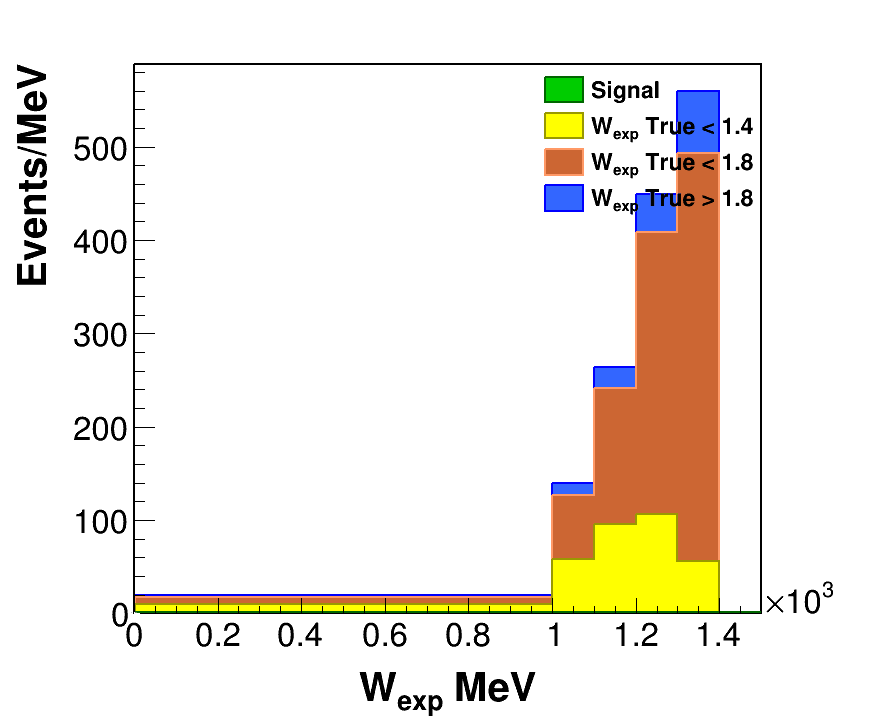
\includegraphics[scale=0.2]{Figures/Chapter4/BGStudies/Bd_Background_wexp_WSB.png}
    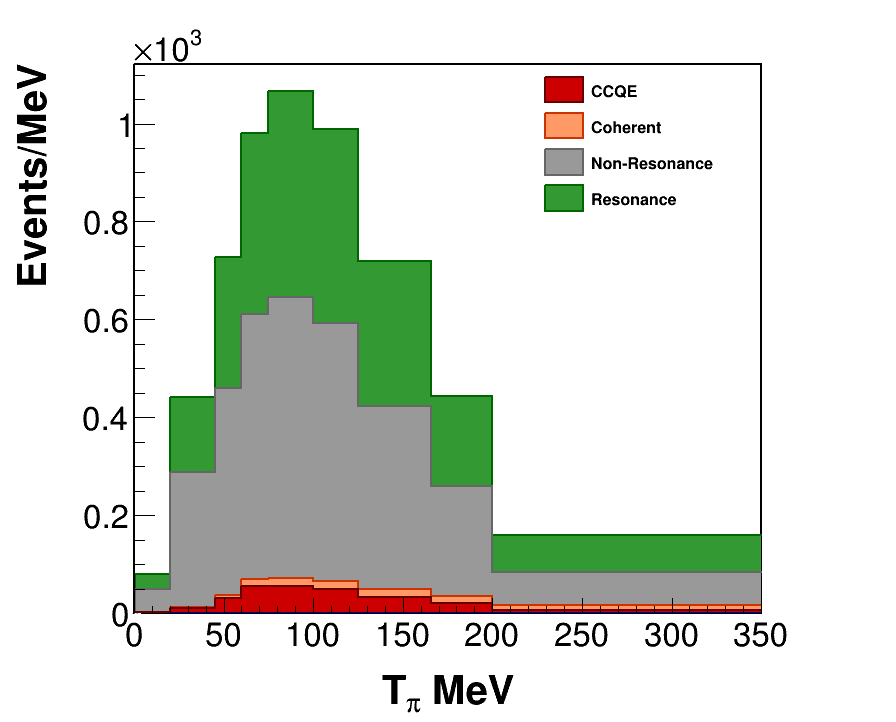
\includegraphics[scale=0.2]{Figures/Chapter4/BGStudies/Bd_Background_mixtpi_Int.png}
    \caption{Breakdown background for $T_\pi$ (left) and $W_{exp}$ (right) variables. The left plot shows the different interactions types that make up the background of the data selection. The right plot shows the background components of the true $W_{exp}$.}
    \label{fig:Analysis:BgStudies:SidebandTunning:BGBreakdownTpiWexp}
\end{figure}



\begin{figure}
    \centering
    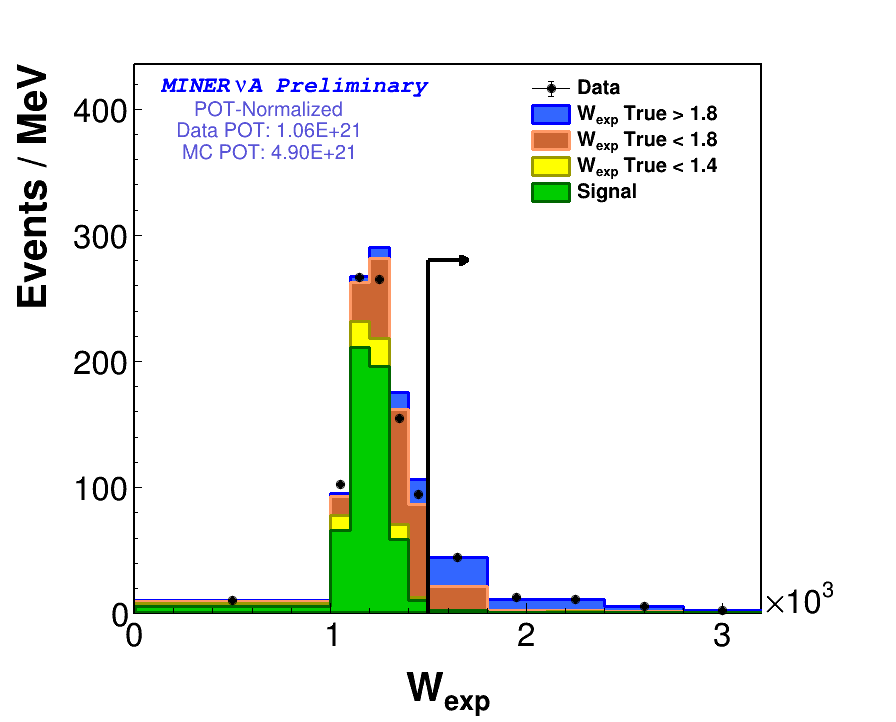
\includegraphics[scale=0.3]{Figures/Chapter4/BGStudies/Breakdown_WSideband_wexp_fit_1Pi_PN_.png}
    \caption{$W_{exp}$ breakdown histogram. This histogram shows the portion of events that are signal }
    \label{fig:enter-label}
\end{figure}


\subsection{Background tuning}

\subsection{Background subtraction}

%++++++++++++++++++++++++++++++++++++++
%     Migration Matrix
%++++++++++++++++++++++++++++++++++++++
\section{Migration Matrix}


%++++++++++++++++++++++++++++++++++++++
%     Ungolding
%++++++++++++++++++++++++++++++++++++++

\section{Unfolding}

\subsection{Warping Studies}

\subsection{Unfolded Distributions}

%++++++++++++++++++++++++++++++++++++++
%     Efficiency  
%++++++++++++++++++++++++++++++++++++++

\section{Efficiency}

\subsection{Efficiency correction}
